\section[Volatility]{Volatility}

Volatility \cite{volatility} is an open-source forensics tool first developed
by Aaron. The four developers of this project also publish the book on memory
forensics, The Art of Memory Forensics.

Volatility is written in Python 2, and the project is being rewritten (2020) in
Python 3. The project is a result of many research in memory forensics in
Windows, Linux, and MacOS. Volatility only works on memory file, and support
many memory file formats.

To find malware in Windows, Volatility has commands to list processes, kernel
modules, inspect the SSDT and IRP, and list unloaded drivers. Volatility also
employs pool tag scanning to find processes, threads, drivers, kernel modules,
network connections, kernel callbacks. Volatility has a command to compare the
process lists produced by traversing different process list and pool tag
scanning for processes, \texttt{psxview}.  Figure \ref{fig:volatility} shows
the sample output of the Volatility's \texttt{psxview} commands.

\begin{figure}[h]
  \centering
  \caption{Volatility}
  \label{fig:volatility}
  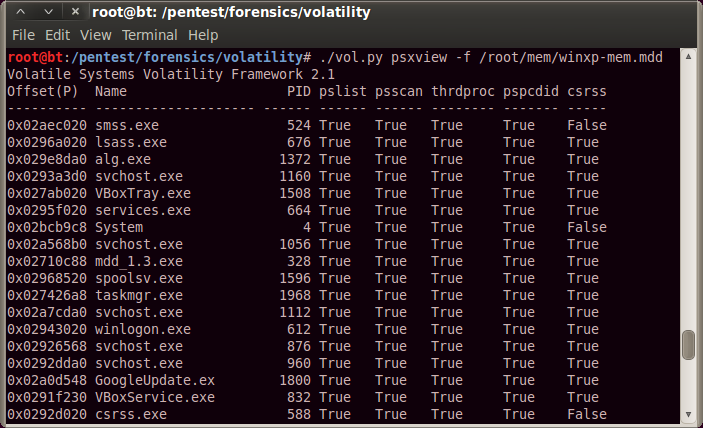
\includegraphics[scale=0.5]{images/volatility.png}
\end{figure}

Volatility is a versatile and powerful tool ever created to tackle the memory
forensics. It can work on memory dumps of different Windows versions and help
investigators explore many data related to the system.
